\section{Tuning of PID controllers using a MOO approach}
\label{PID_Tuning}
The first step to find a suitable tuning rule for \gls{2dof} \gls{pid} controllers for \gls{soptd} plants in a Pareto-optimal sense, is to gather the data. These data was found by applying the \gls{ennc} methodology to problem \eqref{probmoo}, using a normalized version of the plants. Defining the normalized variable $\hat{s}=T s$, then the normalized version of the time delay, $\tau_0$, becomes~\cite{Alfaro2013}:
\begin{equation}
\tau_0 = \frac{L}{T},
\label{eq:tauNorm}
\end{equation}
which allows to find the optimal tuning for a complete family of plants rather than a single plant only. The cases that were computed contained $a$ values from $0$ to $1$ in $0.1$ steps and $\tau_0$ values from $1$ to $2$ in $0.1$ steps and $M_{s,max}=2$. A value of $\tau_0=1$ represents a plant where the time delay is equal to the largest lag time of the system, while in the case of $\tau_0=2$, the time delay is twice the largest lag time. The corresponding normalized PID parameters become:
\begin{equation}
\kappa_p = K_p K, \qquad \tau_i=\frac{T_i}{T}, \qquad \tau_d = \frac{T_d}{T}.
\label{eq:PIDNormParam}
\end{equation}
%

The Pareto front was found for each plant family with around 1000 points each one. Since each point in the Pareto Front represents a different tuning, the number of possible Pareto optimal \gls{pid} controllers found, count to approximately 100 000\footnote{The data base contain other cases beyond the scope of this paper and can be downloaded from \url{http://www2.eie.ucr.ac.cr/~jdrojas/Research/MOOP_PIDTuning/}}.

Once the data is found, the next step is to perform a curve fitting procedure in order to find appropriate equations that match the pattern of the different values of $\kappa_p$, $\tau_i$ and $\tau_d$ as a function of $a$ and $\tau_0$.

In order to determine the PID controller parameters equations for $\kappa_p$, $\tau_i$, $\tau_d$ and $\beta$, a curve fitting procedure was applied. In order to parameterize the tuning rule, the idea of "allowed degradation" is introduced. When $J_{di}$ and $J_{do}$ are normalized as:
%
\begin{align}
\delta &= \frac{J_{di}(\theta)-J_{di, min}(\theta)}{J_{di,max}(\theta)-J_{di,min}(\theta)},\label{eq:delta}\\
\gamma &= \frac{J_{do}(\theta)-J_{do, min}(\theta)}{J_{do,max}(\theta)-J_{do,min}(\theta)},\label{eq:gamma}
\end{align}
%
where both $0 \le \delta \le 1$ and $0 \le \gamma \le 1$, then, a value of $\delta=1$ represents an allowed degradation of 100\% of the response of the controlled system to an input disturbance. Since the data was obtained from the Pareto front of three functions, it is only required to choose the degradation of two functions. If the allowed degradation for both $J_{di}$ and $J_{do}$ are set to $\delta=\gamma=1$, the resulting tuning is expected to represent the optimal tuning for servo control.

Almost two hundred and twenty regressions were run for all considered values of $a$ and $\tau_0$ for every parameter in $\bm{\theta}$. Regression analysis revealed that a second order fit was the most appropriate; as it had an average adjusted R-square of $0.92494$, $0.97997$ and $0.92275$ for $\kappa_p$, $\tau_i$ and $\tau_d$, respectively. First order fits had a poorer adjusted R-square, compared to a second order fit adjusted R-square; except for $\beta$, which was possible to model as a first order function of $\gamma$ and $\delta$, with an average adjusted R-square of $0.96063$. Some results for the corresponding fits of $\kappa_p$, $\tau_i$, $\tau_d$ and $\beta$, is shown in Fig.~\ref{F:cftoolkp}.%, \ref{F:cftoolTd} and \ref{F:cftoolbeta}.   % a second order surface was found to be the best fit for all eleven fits overall, as shown in figure \ref{F:firstfit}.
%
\begin{figure}
	\centering
	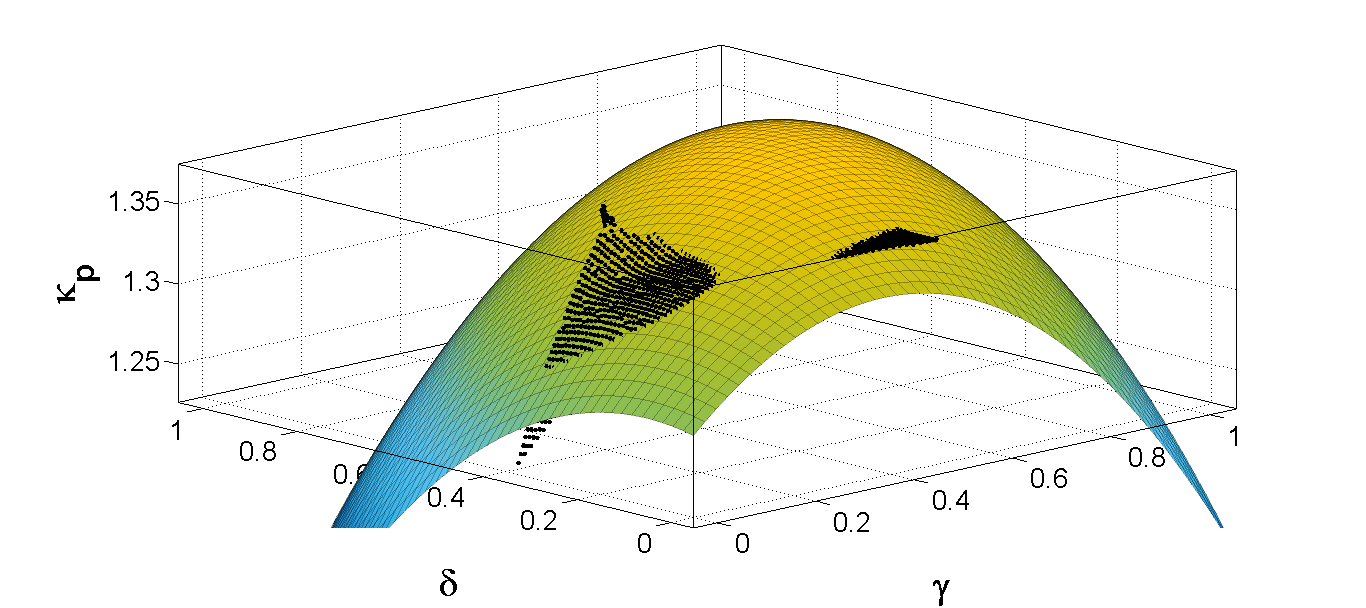
\includegraphics[width=\columnwidth]{kpfit2.png}
	\caption{Second order fit for $\kappa_p$ when $a=0.1$ and $t_{0}=1$}
	\label{F:cftoolkp}
\end{figure}
%
%\begin{figure}
%	\centering
%	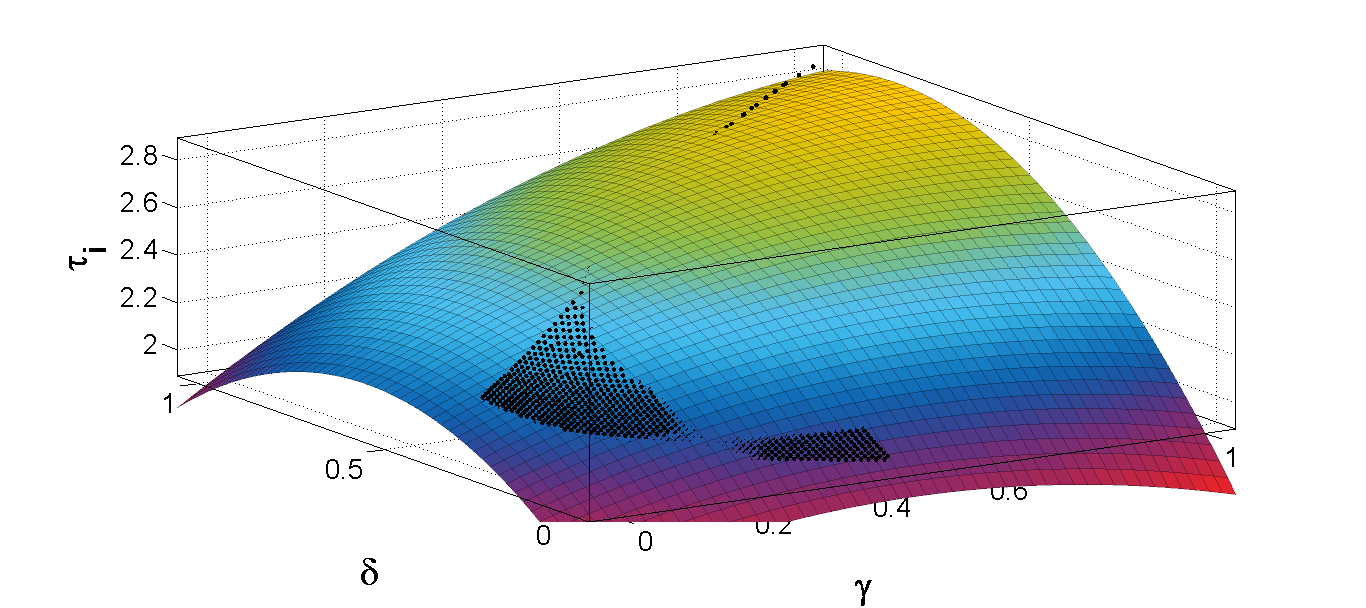
\includegraphics[width=\columnwidth]{Tifit2.png}
%	\caption{Second order fit for $\tau_i$ when $a=0.1$ and $\tau_0=1$}
%	\label{F:cftoolTi}
%\end{figure}
%
%\begin{figure}
%	\centering
%	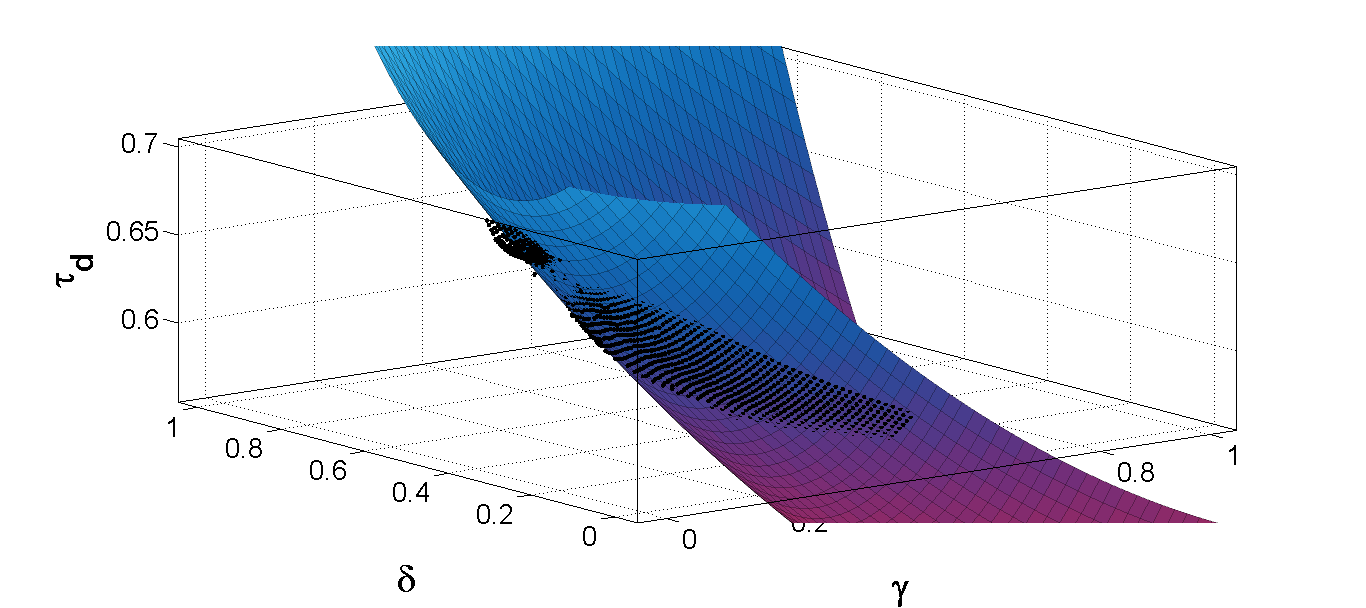
\includegraphics[width=0.5\textwidth]{Tdfit2.png}
%	\caption{Second order fit for $\tau_d$ when $a=0.1$ and $\tau_0=1$}
%	\label{F:cftoolTd}
%\end{figure}
%%
%\begin{figure}
%	\centering
%	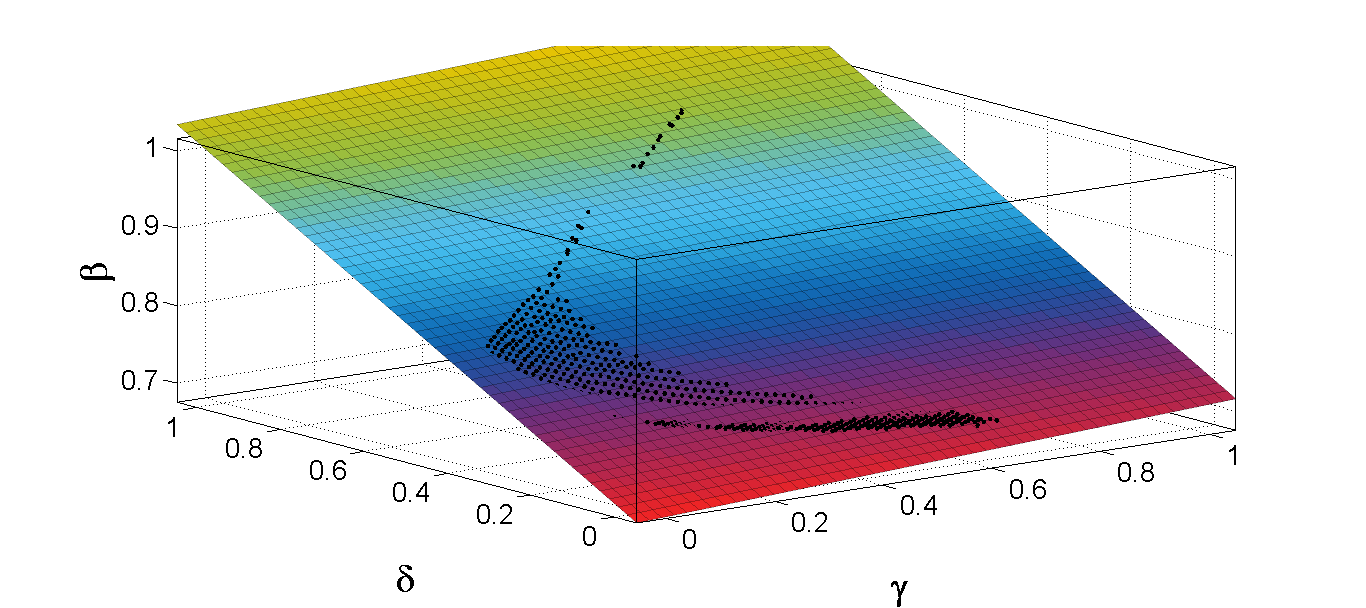
\includegraphics[width=0.5\textwidth]{betafit2.png}
%	\caption{First order fit for $\beta$ when $a=0.1$ and $\tau_0=1$}
%	\label{F:cftoolbeta}
%\end{figure}

The tuning rule for all controller parameters are proposed to be as:  
%
\begin{align}
\kappa_p &= p_{00}+p_{01}\cdot\gamma+p_{02}\cdot\delta\nonumber\\
&\quad + p_{03}\cdot\gamma^2+p_{04}\cdot\gamma\cdot \delta+p_{05}\cdot\delta^2,\label{E:eqkp}\\
%
\tau_i &= p_{10}+p_{11}\cdot\gamma+p_{12}\cdot\delta\nonumber\\
&\quad + p_{13}\cdot\gamma^2+p_{14}\cdot\gamma\cdot \delta+p_{15}\cdot\delta^2,\label{E:eqTi}\\
%
\tau_d &= p_{20}+p_{21}\cdot\gamma+p_{22}\cdot\delta\nonumber\\
&\quad+p_{23}\cdot\gamma^2+p_{24}\cdot\gamma\cdot \delta+p_{25}\cdot\delta^2,\label{E:eqTd}\\
%
\beta &=p_{30}+p_{31}\cdot\gamma+p_{32}\cdot\delta,\label{E:eqbeta}
\end{align}
%

The coefficients $p_{ij}$, where $i=\{0,1,2,3\}$ and $j=\{0,1,2,3,4,5\}$, all vary according to $a$ and $\tau_0$. This dependency suggested to perform another regressions over these parameters in terms of $a$ and $\tau_0$. Therefore a curve fitting procedure was also carried out for every $p_{ij}$. As an example of these regressions, 
%
\begin{figure}
	\centering
	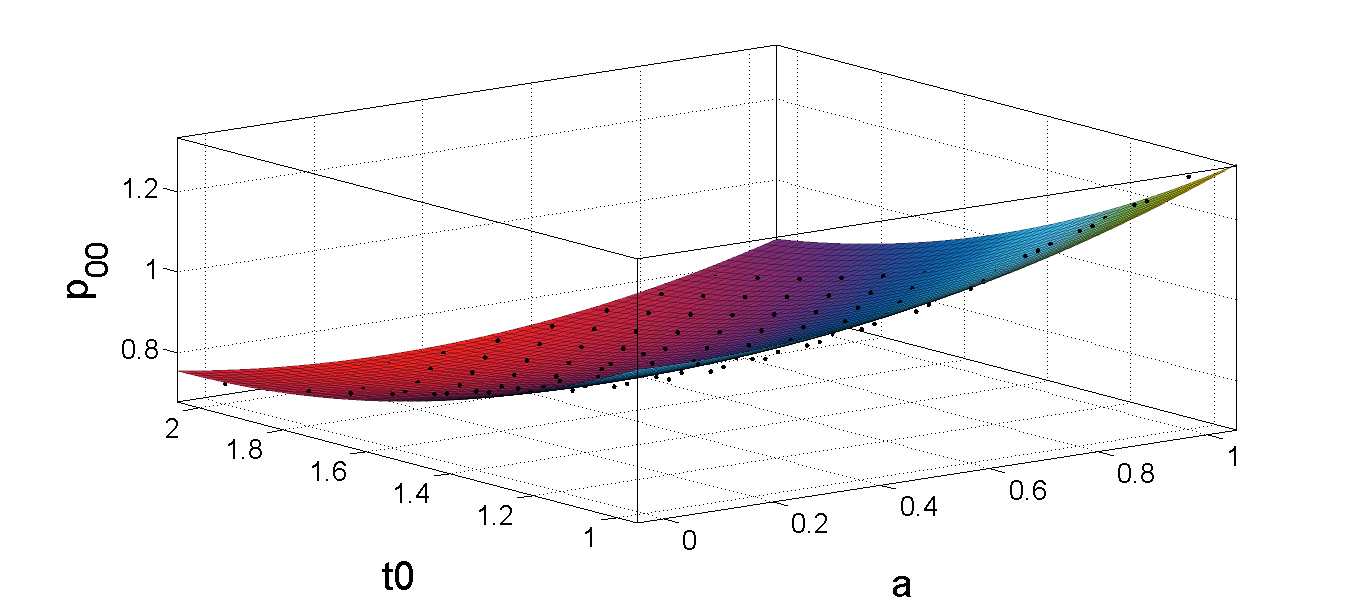
\includegraphics[width=0.8\textwidth]{./a00fit2.png}
	\caption{Second order fit for $p_{00}$ in $\kappa_p$}
	\label{F:coeff}
\end{figure}
%
Fig.~\ref{F:coeff} shows the result for the $p_{00}$ parameter as a function of $a$ and $\tau_0$.  For time-delay dominant process, the values for $\tau_0$ were considered to be in the range such that $1\leq \tau_0 \leq2$. In these cases, the adjusted R-square was higher than $0.9$. It may be possible to find a tuning equation for values of $\tau_0$ from $0.1$ to $2$ , however, this equations may become too complex to achieve a high enough adjusted R-square. This analysis is beyond the scope of this article but will be reported elsewhere.

The most appropriate fit for every coefficient in the range of $1\leq \tau_0 \leq2$, was also a second order fit. The resulting fit is described by:
%
\begin{equation}
p_{ij} = b_{i0}+b_{i1}a+b_{i2} \tau_0+b_{i3}a^2+b_{i4}a \tau_0+b_{i5}\tau_0^2 .
\label{E:coeff}
\end{equation}

Analog to $\bm{\theta}$, two hundred and twenty regressions were made for the coefficients $p_{ij}$, for every parameter in $\bm{\theta}$, except for $\beta$, which had fewer coefficients. The results of the regression analysis for every coefficient for each controller's parameter are shown in Tables~\ref{T:T1}, \ref{T:td}, \ref{T:ti} and \ref{T:beta}.

% Please add the following required packages to your document preamble:
% \usepackage{multirow}
%\begin{table}
%\centering
%\caption{Parameters for $\kappa_p$.}
%\label{T:T1}
%\begin{tabular}{|c|l|l|}
%\hline
%\multicolumn{3}{|c|}{$\kappa_p$ coefficients}           \\ \hline
%$p_{ij}$                  & \multicolumn{2}{c|}{$b_{ik}$} \\ \hline
%\multirow{6}{*}{$p_{00}$} & $b_{00}$      & 1.8203        \\ \cline{2-3} 
%                     & $b_{01}$      & 0.12765       \\ \cline{2-3} 
%                     & $b_{02}$      & -1.0484       \\ \cline{2-3} 
%                     & $b_{03}$      & 0.27085       \\ \cline{2-3} 
%                     & $b_{04}$      & -0.15141      \\ \cline{2-3} 
%                     & $b_{05}$      & 0.25505       \\ \hline
%\multirow{6}{*}{$p_{01}$} & $b_{10}$      & 0.32832       \\ \cline{2-3} 
%                     & $b_{11}$      & 0.22439       \\ \cline{2-3} 
%                     & $b_{12}$      & -0.26761      \\ \cline{2-3} 
%                     & $b_{13}$      & -0.022374     \\ \cline{2-3} 
%                     & $b_{14}$      & -0.068708     \\ \cline{2-3} 
%                     & $b_{15}$      & 0.076273      \\ \hline
%\multirow{6}{*}{$p_{02}$} & $b_{20}$      & 0.29122       \\ \cline{2-3} 
%                     & $b_{21}$      & -0.12878      \\ \cline{2-3} 
%                     & $b_{22}$      & -0.25003      \\ \cline{2-3} 
%                     & $b_{23}$      & 0.10461       \\ \cline{2-3} 
%                     & $b_{24}$      & 0.0048329     \\ \cline{2-3} 
%                     & $b_{25}$      & 0.059478      \\ \hline
%\multirow{6}{*}{$p_{03}$} & $b_{30}$      & 0.042733      \\ \cline{2-3} 
%                     & $b_{31}$      & -0.52048      \\ \cline{2-3} 
%                     & $b_{32}$      & -0.25437      \\ \cline{2-3} 
%                     & $b_{33}$      & 0.47345       \\ \cline{2-3} 
%                     & $b_{34}$      & -0.11069      \\ \cline{2-3} 
%                     & $b_{35}$      & 0.078691      \\ \hline
%\multirow{6}{*}{$p_{04}$} & $b_{40}$      & -0.077455     \\ \cline{2-3} 
%                     & $b_{41}$      & 0.61083       \\ \cline{2-3} 
%                     & $b_{42}$      & 0.24951       \\ \cline{2-3} 
%                     & $b_{43}$      & -0.60316      \\ \cline{2-3} 
%                     & $b_{44}$      & 0.19685       \\ \cline{2-3} 
%                     & $b_{45}$      & -0.071314     \\ \hline
%\multirow{6}{*}{$p_{05}$} & $b_{50}$      & -0.41226      \\ \cline{2-3} 
%                     & $b_{51}$      & -0.24733      \\ \cline{2-3} 
%                     & $b_{52}$      & 0.29554       \\ \cline{2-3} 
%                     & $b_{53}$      & 0.080236      \\ \cline{2-3} 
%                     & $b_{54}$      & 0.013411      \\ \cline{2-3} 
%                     & $b_{55}$      & -0.091089     \\ \hline
%\end{tabular}
%\end{table}
%
\begin{table}
	\centering
	\caption{Coefficients for $\kappa_p$.}
	\label{T:T1}
	\begin{tabular}{@{}cll|cll@{}}
		\hline
		%\multicolumn{6}{c}{$\kappa_p$ coefficients}           \\ \hline
		$p_{ij}$                  & \multicolumn{2}{c}{$b_{ik}$} & $p_{ij}$ & \multicolumn{2}{c}{$b_{ik}$}\\
		\hline
		\multirow{6}{*}{$p_{00}$} & $b_{00}$  & 1.820 &   \multirow{6}{*}{$p_{01}$} & $b_{10}$ & 0.328 \\ % \cline{2-3} \cline{5-6}
		& $b_{01}$      & 0.128   &  	& $b_{11}$      & 0.224 \\ % \cline{2-3} \cline{5-6}
		& $b_{02}$      & -1.048   &	& $b_{12}$      & -0.268 \\ % \cline{2-3} \cline{5-6}
		& $b_{03}$      & 0.270   &	& $b_{13}$      & -0.022 \\ % \cline{2-3} \cline{5-6}
		& $b_{04}$      & -0.151  & 	& $b_{14}$      & -0.069  \\ % \cline{2-3} \cline{5-6}
		& $b_{05}$      & 0.255   &	& $b_{15}$      & 0.076    \\ \hline
		%
		\multirow{6}{*}{$p_{02}$} & $b_{20}$  & 0.291	& \multirow{6}{*}{$p_{03}$} & $b_{30}$ & 0.043 \\ % \cline{2-3} \cline{5-6}
		& $b_{21}$      & -0.129   & & $b_{31}$      & -0.520  \\ % \cline{2-3} \cline{5-6}
		& $b_{22}$      & -0.250   & & $b_{32}$      & -0.254  \\ % \cline{2-3} \cline{5-6}
		& $b_{23}$      & 0.105    & & $b_{33}$      & 0.473   \\ % \cline{2-3} \cline{5-6}
		& $b_{24}$      & 0.005  & & $b_{34}$      & -0.111  \\ % \cline{2-3} \cline{5-6}
		& $b_{25}$      & 0.059   & & $b_{35}$      & 0.079  \\ \hline
		%
		\multirow{6}{*}{$p_{04}$} & $b_{40}$      & -0.077  & \multirow{6}{*}{$p_{05}$} & $b_{50}$      & -0.412   \\ %\cline{2-3} \cline{5-6}
		& $b_{41}$      & 0.611     &  & $b_{51}$      & -0.247\\ %\cline{2-3} \cline{5-6}
		& $b_{42}$      & 0.249     &  & $b_{52}$      & 0.296\\ % \cline{2-3} \cline{5-6}
		& $b_{43}$      & -0.603    &  & $b_{53}$      & 0.080\\ %\cline{2-3} \cline{5-6}
		& $b_{44}$      & 0.197     &  & $b_{54}$      & 0.013\\ % \cline{2-3} \cline{5-6}
		& $b_{45}$      & -0.071   &  & $b_{55}$      & -0.091\\
		\hline
	\end{tabular}
\end{table}

\begin{table}
	\centering
	\caption{Coefficients for $\tau_d$.}
	\label{T:td}
	\begin{tabular}{@{}cll|cll@{}}
		\hline
		%\multicolumn{6}{c}{$\kappa_p$ coefficients}           \\ \hline
		$p_{ij}$                  & \multicolumn{2}{c}{$b_{ik}$} & $p_{ij}$ & \multicolumn{2}{c}{$b_{ik}$}\\
		\hline
		\multirow{6}{*}{$p_{00}$} & $b_{00}$  & 0.111
		&   \multirow{6}{*}{$p_{01}$} & $b_{10}$ & -0.0076
		\\ % \cline{2-3} \cline{5-6}
		& $b_{01}$      & 0.450   &  	& $b_{11}$      & -0.163 \\ % \cline{2-3} \cline{5-6}
		& $b_{02}$      & 0.274   &	& $b_{12}$      & -0.212 \\ % \cline{2-3} \cline{5-6}
		& $b_{03}$      & -0.025   &	& $b_{13}$      & 0.154 \\ % \cline{2-3} \cline{5-6}
		& $b_{04}$      & -0.069  & 	& $b_{14}$      & -0.074  \\ % \cline{2-3} \cline{5-6}
		& $b_{05}$      & 0.003   &	& $b_{15}$      & 0.0026    \\ \hline
		%
		\multirow{6}{*}{$p_{02}$} & $b_{20}$  & -0.238	& \multirow{6}{*}{$p_{03}$} & $b_{30}$ & -0.237 \\ % \cline{2-3} \cline{5-6}
		& $b_{21}$      & 0.105   & & $b_{31}$      & -0.938  \\ % \cline{2-3} \cline{5-6}
		& $b_{22}$      & -0.016   & & $b_{32}$      & 1.121  \\ % \cline{2-3} \cline{5-6}
		& $b_{23}$      & -0.234    & & $b_{33}$      & 0.496   \\ % \cline{2-3} \cline{5-6}
		& $b_{24}$      & 0.094  & & $b_{34}$      & 0.331  \\ % \cline{2-3} \cline{5-6}
		& $b_{25}$      & -0.0254   & & $b_{35}$      & -0.641  \\ \hline
		%
		\multirow{6}{*}{$p_{04}$} & $b_{40}$      & 0.379  & \multirow{6}{*}{$p_{05}$} & $b_{50}$      & -0.224   \\ %\cline{2-3} \cline{5-6}
		& $b_{41}$      & 0.908     &  & $b_{51}$      & 0.109\\ %\cline{2-3} \cline{5-6}
		& $b_{42}$      & -1.330     &  & $b_{52}$      & 0.805\\ % \cline{2-3} \cline{5-6}
		& $b_{43}$      & -1.203    &  & $b_{53}$      & 0.669\\ %\cline{2-3} \cline{5-6}
		& $b_{44}$      & 0.215     &  & $b_{54}$      & -0.527\\ % \cline{2-3} \cline{5-6}
		& $b_{45}$      & 0.683   &  & $b_{55}$      & -0.112\\
		\hline
	\end{tabular}
\end{table}

\begin{table}
	\centering
	\caption{Coefficients for $\tau_i$.}
	\label{T:ti}
	\begin{tabular}{@{}cll|cll@{}}
		\hline
		%\multicolumn{6}{c}{$\kappa_p$ coefficients}           \\ \hline
		$p_{ij}$                  & \multicolumn{2}{c}{$b_{ik}$} & $p_{ij}$ & \multicolumn{2}{c}{$b_{ik}$}\\
		\hline
		\multirow{6}{*}{$p_{00}$} & $b_{00}$  & 0.591
		&   \multirow{6}{*}{$p_{01}$} & $b_{10}$ & -0.408
		\\ % \cline{2-3} \cline{5-6}
		& $b_{01}$      & 0.559   &  	& $b_{11}$      & 0.640 \\ % \cline{2-3} \cline{5-6}
		& $b_{02}$      & 0.545   &	& $b_{12}$      & 0.855 \\ % \cline{2-3} \cline{5-6}
		& $b_{03}$      & 0.017   &	& $b_{13}$      & -0.238 \\ % \cline{2-3} \cline{5-6}
		& $b_{04}$      & 0.045  & 	& $b_{14}$      & -0.0024  \\ % \cline{2-3} \cline{5-6}
		& $b_{05}$      & -0.028   &	& $b_{15}$      & -0.193    \\ \hline
		%
		\multirow{6}{*}{$p_{02}$} & $b_{20}$  & 1.718
		& \multirow{6}{*}{$p_{03}$} & $b_{30}$ & 1.297 \\ % \cline{2-3} \cline{5-6}
		& $b_{21}$      & 0.652   & & $b_{31}$      & -0.423  \\ % \cline{2-3} \cline{5-6}
		& $b_{22}$      & -1.160   & & $b_{32}$      & -2.095  \\ % \cline{2-3} \cline{5-6}
		& $b_{23}$      & -0.855    & & $b_{33}$      & 1.226   \\ % \cline{2-3} \cline{5-6}
		& $b_{24}$      & -0.719  & & $b_{34}$      & -1.041  \\ % \cline{2-3} \cline{5-6}
		& $b_{25}$      & 0.363   & & $b_{35}$      & 0.649  \\ \hline
		%
		\multirow{6}{*}{$p_{04}$} & $b_{40}$      & -0.077  & \multirow{6}{*}{$p_{05}$} & $b_{50}$      & -1.346   \\ %\cline{2-3} \cline{5-6}
		& $b_{41}$      & 0.621     &  & $b_{51}$      & -1.148\\ %\cline{2-3} \cline{5-6}
		& $b_{42}$      & 0.277     &  & $b_{52}$      & 1.224\\ % \cline{2-3} \cline{5-6}
		& $b_{43}$      & -1.193    &  & $b_{53}$      & -0.218\\ %\cline{2-3} \cline{5-6}
		& $b_{44}$      & 1.030     &  & $b_{54}$      & 0.512\\ % \cline{2-3} \cline{5-6}
		& $b_{45}$      & -0.025   &  & $b_{55}$      & -0.572\\
		\hline
	\end{tabular}
\end{table}


\begin{table}
	\centering
	\caption{Coefficients for $\beta$.}
	\label{T:beta}
	\begin{tabular}{@{}cll}
		\hline
		%\multicolumn{6}{c}{$\kappa_p$ coefficients}           \\ \hline
		$p_{ij}$                  & \multicolumn{2}{c}{$b_{ik}$}  \\
		\hline
		\multirow{6}{*}{$p_{00}$} & $b_{00}$  & 0.538
		
		\\ % \cline{2-3} \cline{5-6}
		& $b_{01}$      & 0.023     \\ % \cline{2-3} \cline{5-6}
		& $b_{02}$      & 0.179   	\\ % \cline{2-3} \cline{5-6}
		& $b_{03}$      & -0.114    \\ % \cline{2-3} \cline{5-6}
		& $b_{04}$      & 0.047   	  \\ % \cline{2-3} \cline{5-6}
		& $b_{05}$      & -0.034   \\ \hline
		%
		\multirow{6}{*}{$p_{01}$} & $b_{10}$  & -0.152
		\\ % \cline{2-3} \cline{5-6}
		& $b_{11}$      & 0.065    \\ % \cline{2-3} \cline{5-6}
		& $b_{12}$      & 0.277      \\ % \cline{2-3} \cline{5-6}
		& $b_{13}$      & 0.017      \\ % \cline{2-3} \cline{5-6}
		& $b_{14}$      & -0.052   \\ % \cline{2-3} \cline{5-6}
		& $b_{15}$      & -0.082     \\ \hline
		%
		
		\multirow{6}{*}{$p_{02}$} & $b_{20}$  & 0.585
		\\ % \cline{2-3} \cline{5-6}
		& $b_{21}$      & -0.082    \\ % \cline{2-3} \cline{5-6}
		& $b_{22}$      & -0.280      \\ % \cline{2-3} \cline{5-6}
		& $b_{23}$      & 0.116      \\ % \cline{2-3} \cline{5-6}
		& $b_{24}$      & 0.011   \\ % \cline{2-3} \cline{5-6}
		& $b_{25}$      & 0.044     \\ \hline
		%
		
	\end{tabular}
\end{table}
%
\subsection{Comparison of regression results vs. ENCC results}

After setting up the proposed equations for $\bm{\theta}$, simulations were run to compare the original data against the proposed methodology. The test plant is modeled as: 

\begin{equation}
P_1(s) = \frac{e^{-1.5\hat{s}}}{(\hat{s}+1)(0.5\hat{s}+1)}
\label{E:P1}
\end{equation}

Where $K=1$, $T=1$ s, $L=1.5$ s and $a = 0.5$. 
Table \ref{T:comparison} shows a comparison between the results of the tuning from the MOO problem against the results of using the proposed tuning, where the values for $\delta$ and $\gamma$ were chosen to be the worst case scenario for both $J_{do}$ and $J_{di}$, so $\delta=1$ and $\gamma=1$. 
%
\begin{table}
	\centering
	\caption{Comparison of the \gls{ennc} \gls{moo} data vs. fitted data, using $\delta = 1$ and $\gamma = 1$.}
	\label{T:comparison}
	\begin{tabular}{@{}K{0.25\columnwidth} K{0.25\columnwidth} K{0.25\columnwidth}@{}}
		\toprule
		$\bm{\theta}$ parameters and IAEs & ENCC Method & Fitted data\\
		\midrule
		$\kappa_p$	& $0.810$	& $0.793$ \\
		$\tau_i$	& $2.176$ s	& $2.113$ s	\\
		$\tau_d$	& $0.644$ s	& $0.720$ s \\
		$\beta$		& $1.000$	& $1.000$ \\
		$J_r$		& $2.689$ 	& $2.691$ \\
		$J_{di}$ 	& $2.687$ 	& $2.673$ \\
		$J_{do}$	& $2.689$	& $2.691$ \\
		$M_s$		& $1.9174$	& $1.9449$\\
		\bottomrule
	\end{tabular}
\end{table} 

As it can be seen from Table \ref{T:comparison}, results obtained from the proposed tuning rule are very similar to those obtained from the \gls{ennc} \gls{moo} method. Plots for each method were drawn as shown in Fig.~\ref{F:firstsim}.
%%%ESTA FIGURA HAY QUE CENTRARLA MEJOR
%
\begin{figure}
	\centering
	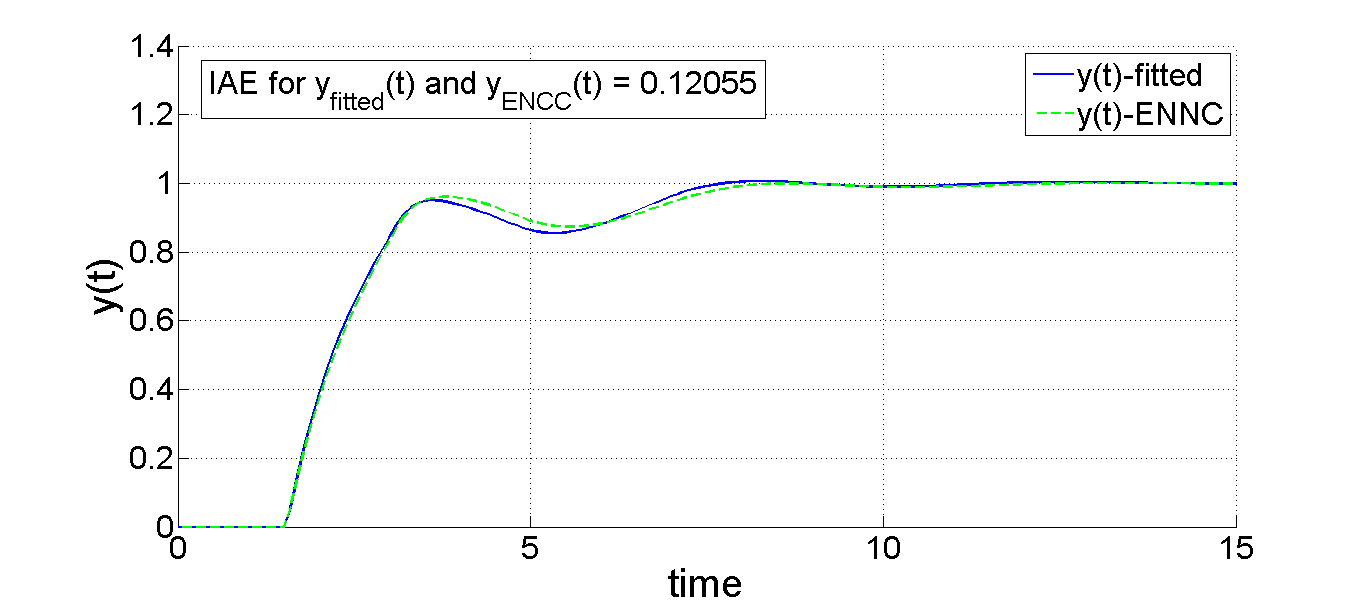
\includegraphics[width=0.8\columnwidth]{servo2.png}
	\caption{Servo response for the ENCC results and regressions results.}
	\label{F:firstsim}
\end{figure}
%
The response of the control signal is given in Fig.~\ref{F:u1}.
%
\begin{figure}
	\centering
	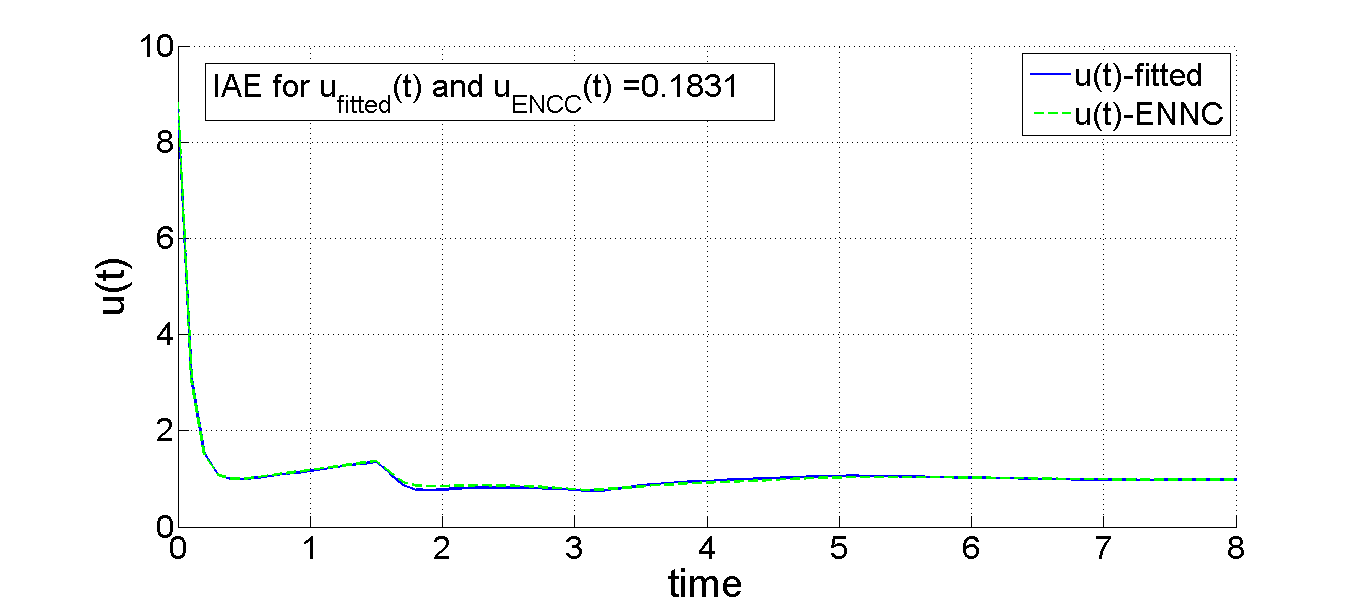
\includegraphics[width=0.8\columnwidth]{u2.png}
	\caption{Control action response for ENCC results and regressions, for a reference step change.}
	\label{F:u1}
\end{figure}

The comparison of the response to an input-disturbance is presented in Fig.~\ref{F:di1}. The error between the proposed methodology and the \gls{moo} results has an \gls{iae} of $0.08$, showing that the polynomial equations are able to encapsulate the optimal tuning of the parameters. In Fig.~\ref{F:do1}, the response to the output disturbance is presented and, as it can be seen, the match is good as well, with an \gls{iae} value of $0.12$.
%
\begin{figure}
	\centering
	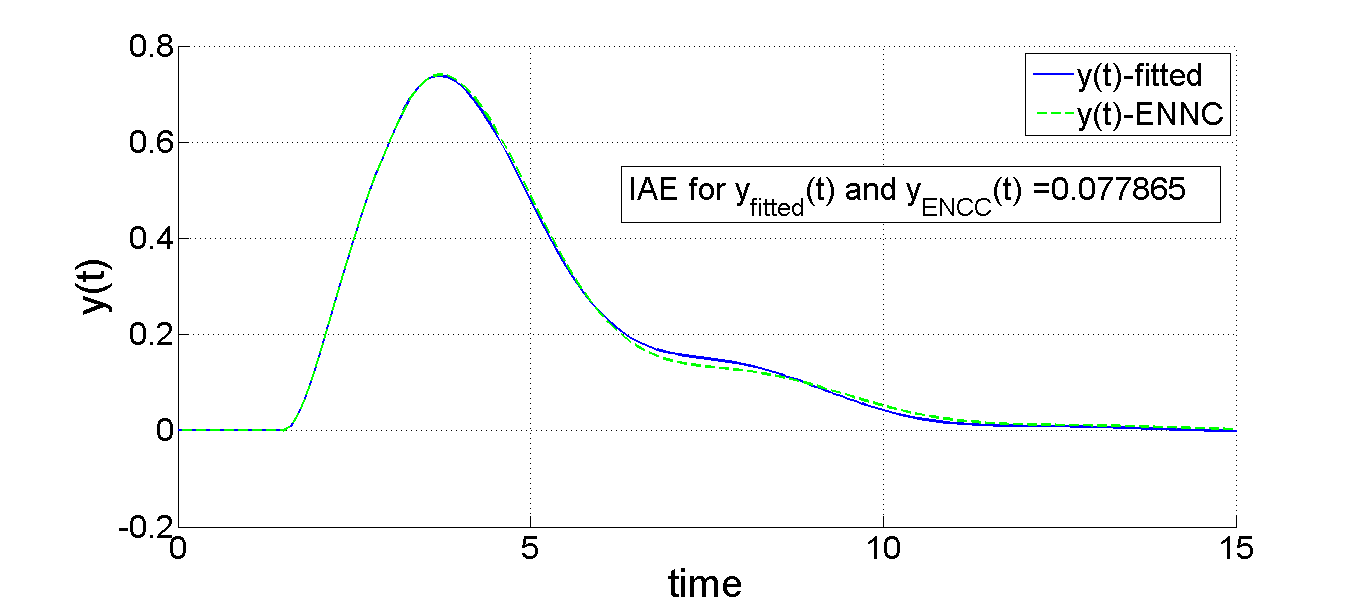
\includegraphics[width=0.8\columnwidth]{di2.png}
	\caption{Step input disturbance response for ENNC results and regressions results.}
	\label{F:di1}
\end{figure}
%
\begin{figure}
	\centering
	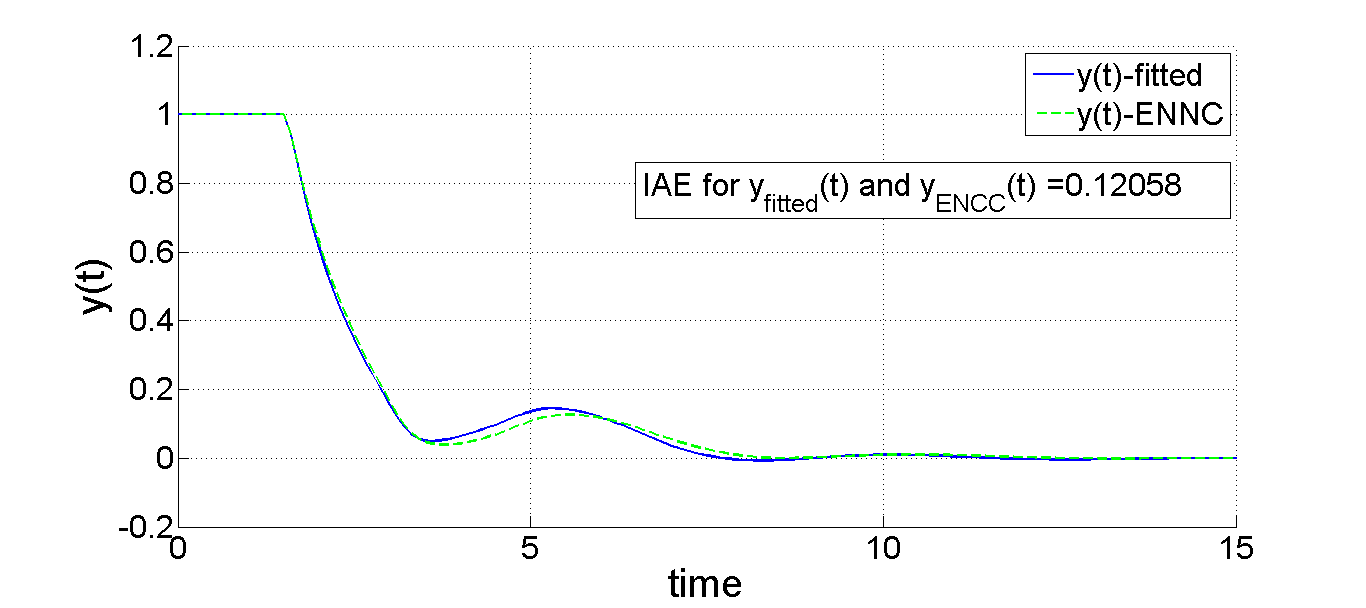
\includegraphics[width=0.8\columnwidth]{do2.png}
	\caption{Step output disturbance response for ENNC results and regressions results.}
	\label{F:do1}
\end{figure}
%

From this example, it is clear that the obtained polynomial equations effectively reproduce the behavior of the parameters found from the ENNC optimization.

The method is also tested for the extreme case scenarios for $\tau_0$ ($\tau_0=1$ and $\tau_0=2$), as given by the models:
%
\begin{equation}
P_F(\hat{s}) = \frac{e^{-\hat{s}}}{(\hat{s}+1)(0.5\hat{s}+1)},
\label{E:p2}
\end{equation}
%
\begin{equation}
P_S(\hat{s}) = \frac{e^{-2\hat{s}}}{(\hat{s}+1)(0.5\hat{s}+1)},
\label{E:p3}
\end{equation}
%
where $P_F(\hat{s})$ and $P_S(\hat{s})$ stand for the fastest and slowest time-delayed dominant test-bench plants, respectively.

For each of these plants, it was established that $\delta = 0.5$ and $\gamma = 0.5$, which is an intermediate case for degradation for both $\delta$ and $\gamma$ in the Pareto front. Results for $J_r$ for $P_F$ and $P_S$ are shown in Table \ref{T:T2}.

\begin{table}
	\centering
	\caption{Results for $J_{di}$, $J_{do}$ and $J_{r}$, using $\delta = 0.5$ and $\gamma = 0.5$.}
	\label{T:T2}
	\begin{tabular}{@{}K{0.25\columnwidth} K{0.25\columnwidth} K{0.25\columnwidth}@{}}
		\toprule
		$\bm{\theta}$ and IAE & For $P_F(s)$ & For $P_S(s)$\\
		\midrule
		$\kappa_p$	& $1.150$ 	& $0.742$ \\
		$\tau_i$ 	& $1.987$ s & $2.345$ s \\
		$\tau_d$ 	& $0.425$ s & $0.629$ s \\
		$\beta$ 	& $0.887$ 	& $0.919$ \\
		$J_r$ 		& $1.955$ 	& $3.360$ \\
		$J_{di}$ 	& $1.729$ 	& $3.162$ \\
		$J_{do}$ 	& $1.874$ 	& $3.237$ \\
		$M_s$		& $2.024$	& $1.976$ \\
		\bottomrule
	\end{tabular}
\end{table} 
%

From these examples, it is clear that the proposed methodology is able to produce Pareto-optimal controllers, for a large set of plants. The obtained dynamical response can be easily changed by the control engineer and, if the selection of $\delta$ and $\gamma$ is appropriate, the controller parameters are likely to produce a closed-loop system with a maximum sensitivity such that $M_s \leq 2$. The principal characteristic of the proposed methodology, is its ability to let the user select the dynamical behavior, taking into account multiple sources of disturbances, unlike other \gls{pid} tuning rules.

\subsection{Comparison of proposed tuning rule against uSORT2 tuning rule}
%
Servo and disturbance responses were obtained for the test-bench plant in \eqref{E:P1}, by using the proposed tuning rule, and then, by using the uSORT2 tuning method for \gls{2dof} \gls{pid} controllers. The objective is to compare both rules to see which one is more flexible in terms of robustness and performance. The uSORT2 method was selected for comparison given that it minimizes $J_{di}$ and find a sub-optimal solution for $J_r$ while keeping $M_s=2$.
%
%Three cases were considered, one in which $\delta$ and $\gamma$ were maximum as in the comparison made in Table~\ref{T:T4}, and the others were when $\delta$ and $\gamma$ have their minimum achievable value for the obtained Pareto front as in Table~\ref{T:T5} and Table~\ref{T:T6}.

Two cases were considered, one in which $\delta$ and $\gamma$ were maximum as in the comparison made in Table~\ref{T:T4}, and the others were when $\delta$ and $\gamma$ have their minimum achievable value for the obtained Pareto front as in Table~\ref{T:T5}.
%%
\begin{table}
	\centering
	\caption{Result comparison of the proposed tuning rule vs. uSORT2 tuning rule, using $\delta = 1$ and $\gamma = 1$.}
	\label{T:T4}
	\begin{tabular}{@{}K{0.25\columnwidth} K{0.25\columnwidth} K{0.25\columnwidth}@{}}
		\midrule
		$\bm{\theta}$ and IAEs & Proposed tuning rule & uSORT2 tuning rule \\
		\midrule
		$\kappa_p$ & 0.793 & 0.814 \\
		$\tau_i$ & 2.113 s & 1.676 s \\
		$\tau_d$ & 0.720 s & 0.775 s \\
		$\beta$ & 1.000 & 0.788 \\
		$J_r$ & 2.691 & 2.692 \\
		$J_{di}$ & 2.673 & 2.290 \\
		$J_{do}$ & 2.691 & 2.451 \\
		$M_{s}$ & 1.945 & 2.007 \\
		\bottomrule
	\end{tabular}
\end{table} 
%
\begin{table}
	\centering
	\caption{Comparison of the proposed tuning rule vs. uSORT2 tuning rule, using $\delta = 0.302$ and $\gamma = 0$.}
	\label{T:T5}
	\begin{tabular}{@{}K{0.25\columnwidth} K{0.25\columnwidth} K{0.25\columnwidth}@{}}
		\midrule
		$\bm{\theta}$ parameters and IAEs & Proposed tuning rule & uSORT2 tuning rule \\
		\midrule
		$\kappa_p$ & 0.820 & 0.814 \\
		$\tau_i$ & 1.808 s & 1.676 s \\
		$\tau_d$ &  0.670 s & 0.775 s \\
		$\beta$ & 0.8261 & 0.788 \\
		$J_r$ & 2.653 & 2.692 \\
		$J_{di}$ & 2.307 & 2.290 \\
		$J_{do}$ & 2.431 & 2.451 \\
		$M_{s}$ & 1.935 & 2.007 \\
		\bottomrule
	\end{tabular}
\end{table}
%%
%\begin{table}
%\centering
%\caption{Result comparative of the proposed tuning rule vs. uSORT2 tuning rule, using $\delta = 0$ and $\gamma = 0.208$.}
%\label{T:T6}
%\begin{tabular}{@{}K{0.25\columnwidth} K{0.25\columnwidth} K{0.25\columnwidth}@{}}
%\midrule
%$\bm{\theta}$ parameters and IAEs & Proposed tuning rule & uSORT2 tuning rule \\
%\midrule
%$\kappa_p$ & 0.855 & 0.814 \\
%$\tau_i$ & 1.762 s & 1.676 s \\
%$\tau_d$ &  0.604 s & 0.775 s \\
%$\beta$ & 0.763 & 0.788 \\
%$J_r$ & 2.573 & 2.692 \\
%$J_{di}$ & 2.143 & 2.290 \\
%$J_{do}$ & 2.484 & 2.451 \\
%$M_{s}$ & 1.980 & 2.007 \\
%\bottomrule
%\end{tabular}
%\end{table}
%%
%%
\begin{figure}
	\centering
	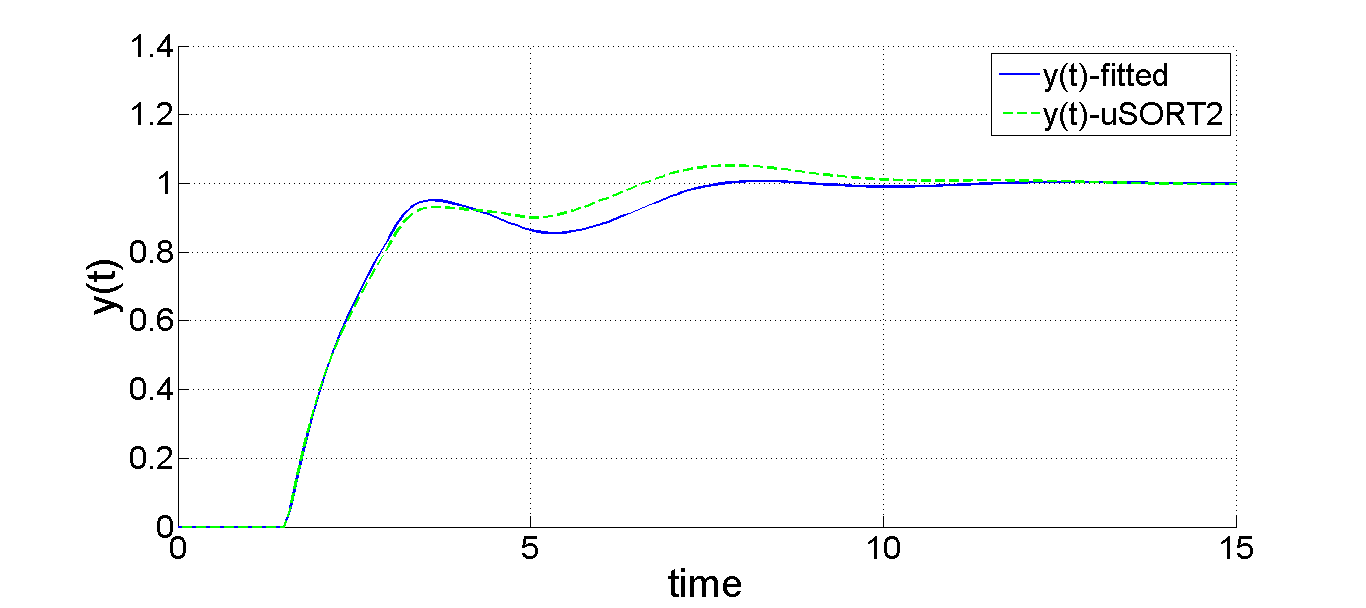
\includegraphics[width=0.8\columnwidth]{./uSORT2.png}
	\caption{Servo input response for both proposed rule and uSORT2 rule.}
	\label{F:uSort}
\end{figure}
%%
%From the results obtained in Tables \ref{T:T4}, \ref{T:T5} and \ref{T:T6},
It is clear that for the two different variations of $\delta$ and $\gamma$, the minimum \gls{iae} for servo response was obtained according to the Pareto front. Also it is important to note that, for the proposed tuning rule, although variations of $\delta$ and $\gamma$ were performed, the maximum sensitivity remained under the value of $M_s \leq 2.0$. This means that given any two inputs within the established Pareto front, the proposed tuning rule gives the optimized value for $J_r$ and it manages to maintain the controller robustness. On the other hand, the uSORT2 tuning rule only focuses on the latter. %For the three given cases in tables \ref{T:T4}, \ref{T:T5} and \ref{T:T6}, the proposed tuning rule proves to be versatile not only in terms of robustness, but also in terms of performance choice.
The uSORT2 methodology provides excellent results, but it is focused on optimizing $J_{di}$. The proposed methodology, although more complex in its equations, gives the control engineers, the freedom to mold the dynamic response to their needs. As an example, the servo response of the controlled system with the proposed methodology and the uSORT is presented in Fig.~\ref{F:uSort}